\section{Sculptures and HDA}

    The above mappings do not provide us with a procedure for deciding whether an higher-dimensional automaton, even finite, is a sculpture, because the bulk can be of any dimension, hence there are infinitely many embeddings to check. There is an alternative way of translating higher-dimensional automata into ST-structures that works on paths starting from the shortest path in the initial cell, essentially unfolding the higher-dimensional automaton.
    % This method is essentially the one used in \cite[Def.3.39]{Johansen16STstruct}, with a few simplifications and greater care taken for the notion of equivalence of events, which is essential for our purposes here.

    \begin{definition}[$\allHDA$ to $\allST$ through paths]
        \label{def:HDA-to-ST-paths}
        Define a map $\hintost:\allHDA\rightarrow\allST$ which builds an ST-structure $\hintost(\mathcal{H})$ by associating to each rooted path $\pi\in \mathcal{H}$ an ST-configuration as follows.
        \begin{enumerate}
            \item\label{hintost_1} for the minimal rooted path, which ends in $\mathcal{I}$, associate $(\emptyset,\emptyset)$;

            \item\label{hintost_2} for any path $\pi=\pi_{s}\transition{s}q_{1}$ that ends in a transition $\finishPath{\pi}=q_{1}\in \mathcal{Q}_{1}$ then 
            \begin{enumerate}
                \item\label{hintost_21} add the ST-configuration $\hintost(\pi)=\hintost(\pi_{s})\cup(q_{1},\emptyset)$;
                \item\label{hintost_22} add the ST-configuration $\hintost(\pi\transition{t}q_{0})=\hintost(\pi)\cup(\emptyset,q_{1})$;
            \end{enumerate}

            \item\label{hintost_3} for any path $\pi$ that ends in a higher cell $\finishPath{\pi}=q_{n}\in \mathcal{Q}_{n}$, with $n\geq 2$, then add the ST-configuration $\hintost(\pi)=\hintost(\pi^{i}) \cup \hintost(\pi^{j})$, with $\pi^{i} \neq \pi^{j}$, $\pi^{i}\transition{s}q_{n}$, and $\pi^{j}\transition{s}q_{n}$.
        \end{enumerate}
 
        % % \cjlong{Definition on cells instead of paths.}
        % Define a map $\hintost:\allHDA\rightarrow\allST$ which builds an ST-structure $\hintost(H)$ by associating to each cell an ST-configuration based on paths as follows.
        % \begin{enumerate}
            % \item\label{hintost_1} for the initial cell $I$ associate $\hintost(I)=(\emptyset,\emptyset)$;
 
 
            % \item\label{hintost_2} for any transition $q_{1}\in Q_{1}$ consider the shortest path $\pi$ s.t.\ $\pi_{s}\transition{s}q_{1} = \pi$ then 

            % \begin{enumerate}
                % \item\label{hintost_21} add the ST-configuration $\hintost(\finishPath{\pi})=\hintost(\finishPath{\pi_{s}})\cup(q_{1},\emptyset)$,
 
                % \item\label{hintost_22} add the ST-configuration $\hintost(\finishPath{\pi\transition{t}q_{0}})=\hintost(\finishPath{\pi})\cup(\emptyset,q_{1})$;
            % \end{enumerate}
 
 
            % \item\label{hintost_3} for any higher cell $q_{n}\in Q_{n}$, with $n\geq 2$, and two paths $\pi^{i}\neq\pi^{j}$, $\pi^{i}\transition{s}q_{n}$, and $\pi^{j}\transition{s}q_{n}$, then add the ST-configuration $\hintost(q_{n})=\hintost(\finishPath{\pi^{i}})\cup\hintost(\finishPath{\pi^{j}})$.
        % \end{enumerate}
    \end{definition}
    
    Note that in the case~\ref{hintost_3} above the paths $\pi^{i},\pi^{j}$ always exist because we work with non-selflinked $\HDA$s. 
    %The same goes for the path $\pi_{s}$ used in \ref{hintost_21}.
    All cells are reachable through the paths considered in the above definition when applied inductively on the length of the distance from the initial cell.
    
<<<<<<< HEAD
        
    \ctlong{Broken box example from Ch.4 moved here.}
=======
    For every transition we add one new event to the ST-structure. This adds too many events and does not capture the geometrical intuitions about concurrency, where transitions parallel in the sides of a filled square should represent the same event. Indeed, the construction is similar to an \emph{unfolding}~\cite{Fahrenberg15PartialHDA}, except that no homotopy equivalence is applied. See~\cite[Def.~3.39]{Johansen16STstruct} for a related construction.
    
    If we are faced with an HDA which may or may not be a sculpture, then there is a minimal equivalence on its transition cells, which is exactly the equivalence of two cells appearing as opposite faces of a square, and the transitive closure.
    
    \begin{definition}[Events equivalence relation of $\HDA$ \cite{Johansen16STstruct}]
        Define a relation $\eventEquivHDAs\ \subseteq \mathcal{Q}_{1}\times \mathcal{Q}_{1}$ on transitions of $\mathcal{H}$ as 
        
        \[
            q_{1}\eventEquivHDAs q_{1}' \quad\text{iff}\quad \exists q_{2}\in
            \mathcal{Q}_{2}:\alpha_{i}(q_{2})=q_{1}\wedge \beta_{i}(q_{2})=q_{1}'
        \]
        for some $i\leq 2$ and $\alpha,\beta\in\{s,t\}$.  Consider the reflexive and transitive closure of the above relation, and denote it the same. This is now an equivalence relation on $\mathcal{Q}_{1}$.
        % Consider an equivalence class $\equivClass{q_{1}}$ to be all
        % $q_{1}'$ equivalent with $q_{1}$.  Such an equivalence class is
        % called \emph{an event}.
    \end{definition}
    
    In Section \ref{sec:st-structure-and-hda}, we had already defined the events equivalence relation of $\HDA$ when defining a mapping from $\allHDA$ to $\allST$.
>>>>>>> 6a85ddbdff57f2fe030ed38810e4ef49c2b1c3cd
    
    As shown in \cite[Proposition 3.42]{Johansen16STstruct}, the mapping $\ST$ associates an acyclic and non-degenerate higher-dimensional automata with $\ST(H)$, which is a rooted, connected, and adjacent-closed ST-structure. The mapping $\ST$ from Definition~\ref{def:HDA-to-ST-structure} preserves isomorphism of reachable parts. However, it may collapse non-isomorphic higher-dimensional automata into isomorphic ST-structures. This can be seen by considering the two higher-dimensional automata from Figure \ref{fig:HDA-broken-box}, which are translated into the same ST-structure by $\ST$. The mapping $\ST$ considers the two higher-dimensional automata which are not isomorphic to be two ST-structures which are isomorphic. The higher-dimensional automata are not isomorphic since the left one has a split corner whereas the right one is a cube with its faces nicely placed, forming a complete cube.

    %This can be seen by considering the two higher-dimensional automata from Figure~\ref{fig:HDA-broken-box} without the two dotted transitions, which are translated into the same ST-structure by $\ST$. Even when the dotted transitions are added, they are mapped to the same ST-structure.

    \begin{example}[Broken box example]\label{exp:hda-broken-box}
        This example is taken from \cite[Section 9.2.1]{Glabbeek06HDA}, and also found illustrated in \cite[Figure 6]{Johansen16STstruct}. As part of van Glabbeek's presentation at EXPRESS 2004, the process displayed in Figure \ref{fig:HDA-broken-box} (left) was demonstrated with the help of the audience. We name the Figure \ref{fig:HDA-broken-box} (left) for the broken box since it represent a higher-dimensional automaton which looks almost like a complete cube, but with a single corner split.
    
        \begin{figure}[ht]
            \centering
            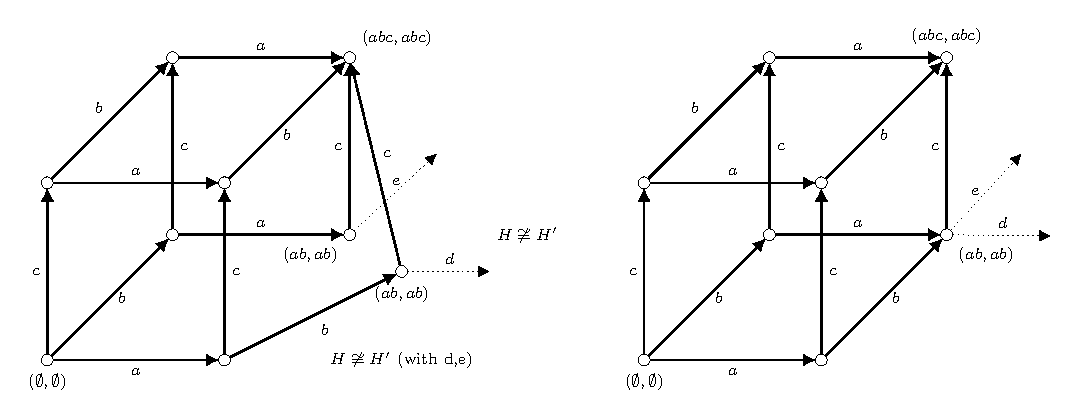
\includegraphics[scale=0.9]{Figures/5.Relationship-with-other-models-of-true-concurrency/broken_box(figure_6_left)/HDA-broken-box.pdf}
            \captionof{figure}[Broken box]{Example of ST-structures and higher-dimensional automata representing the broken box example. The ST-structure (left) is isomorphic to ST-structure (right). On the other hand, we see the higher-dimensional automaton (left) is not isomorphic to the higher-dimensional automaton (right). Since, the higher-dimensional automaton (left) has a split corner and the higher-dimensional automaton (right) is a nicely shaped cube.}
            \label{fig:HDA-broken-box}
        \end{figure}
    
        The example was of two computer scientists $A$ and $B$ travelling from one end of the podium to the other. Their task was to perform the actions $a$ and $b$, respectively, of crossing a line on the podium. Due to strategic placing of obstacles, the only place where this was possible was at a narrow opening between the obstacles that had room for only one of the scientist $A$ and $B$ at a time. This made the action $a$ and $b$ mutually exclusive, in the sense that they could not occur simultaneously.
    
        A third computer scientist $C$, was assigned the task $c$ of removing an obstacle that caused the bottleneck to exist. The action $c$ was executed causally independent of $a$ and $b$, that is, a and b are concurrent. The actions $a$ and $b$ were mutually exclusive only until $c$ occurred, after which they became causally independent.
    
        Finally, a fourth participant was assigned the task of making a statement when $a$ and $b$ had both occurred before the action $c$ started. This statement was going to be $d$ in case $A$ passed the bottleneck before $B$ did, and $e$ in case $B$ passed the bottleneck before $A$ did. Hearing this statement would prevent computer scientist $C$ from carrying out action $c$.
    
        The ST-structures of Figure \ref{fig:HDA-broken-box} (left and right) are isomorphic. However, we see the higher-dimensional automaton of Figure \ref{fig:HDA-broken-box} (left) is not isomorphic to the higher-dimensional automaton of Figure \ref{fig:HDA-broken-box} (right).
    \end{example}

    The mapping $\ST$ from Definition \ref{def:HDA-to-ST-structure} preserve isomorphism. However, it may collapse non-isomorphic higher-dimensional automata into isomorphic ST-structures. Consider the two higher-dimensional automata from Figure \ref{fig:HDA-broken-box} which are not isomorphic since the left one has a split corner whereas the right one is a cube with nicely placed faces, but the ST-structures that the mapping $\ST$ associates are isomorphic. This means that $\ST$ is not an embedding from $\allHDA$ to $\allST$ since it looses information, which is the mappings ability to announce the difference between when $A$ happens before $B$ or $B$ happens before $A$. In other words, being able to see the difference between the split corner of a cube and a nicely shaped cube.


    
    \begin{theorem}
        \label{th:non-sculpting}
        Not all $\HDA$ are sculptures.
    \end{theorem}
    
    \begin{proof}
        Use the definition of $\allHDA$ to $\allST$ through paths to show the broken box example is not a sculpture.
    \end{proof}